\chapter{Concept Drift Detection}
\label{exp1}
\section{Data Used}

The whole dataset was collected by web crawler, containing 181903 fashion news in www.hypebeast.com from 20/04/2005 to 13/06/2018. A sample of the dataset including the date of the publication, the category, the keywords, the title, the context, the HYPES, and the class of the HYPES. The HYPES is the real time popularity metric informing reader of what is trending. The HYPES is computed based on the page-viewers, the comments, and the information flow on social network. The HYPES is classified into 3 classes which is shown in Table \ref{popularityclasses} of the introduction chapter. 

During the development of the website, HYPEBEAST also changed the algorithm of computing the HYPES. Figure \ref{hypes_yeas} shows the change of the HYPES from 2015 to 2018. And the distribution of each class over the past 13 years is presented in Figure \ref{proportion_yeas}. It is obvious that after the middle of 2013, HYPES have a significant jump and the present a rising trend until 2018. However, the proportions of classes remain stable after 2014. Based on this intuitive analysis, we select the data from 01/01/2014 to 13/08/2018 as the dataset for the experiment. It containing 95787 fashion news. The distribution of the classes is shown in Table \ref{distribution_classes}

\begin{figure}
\centering
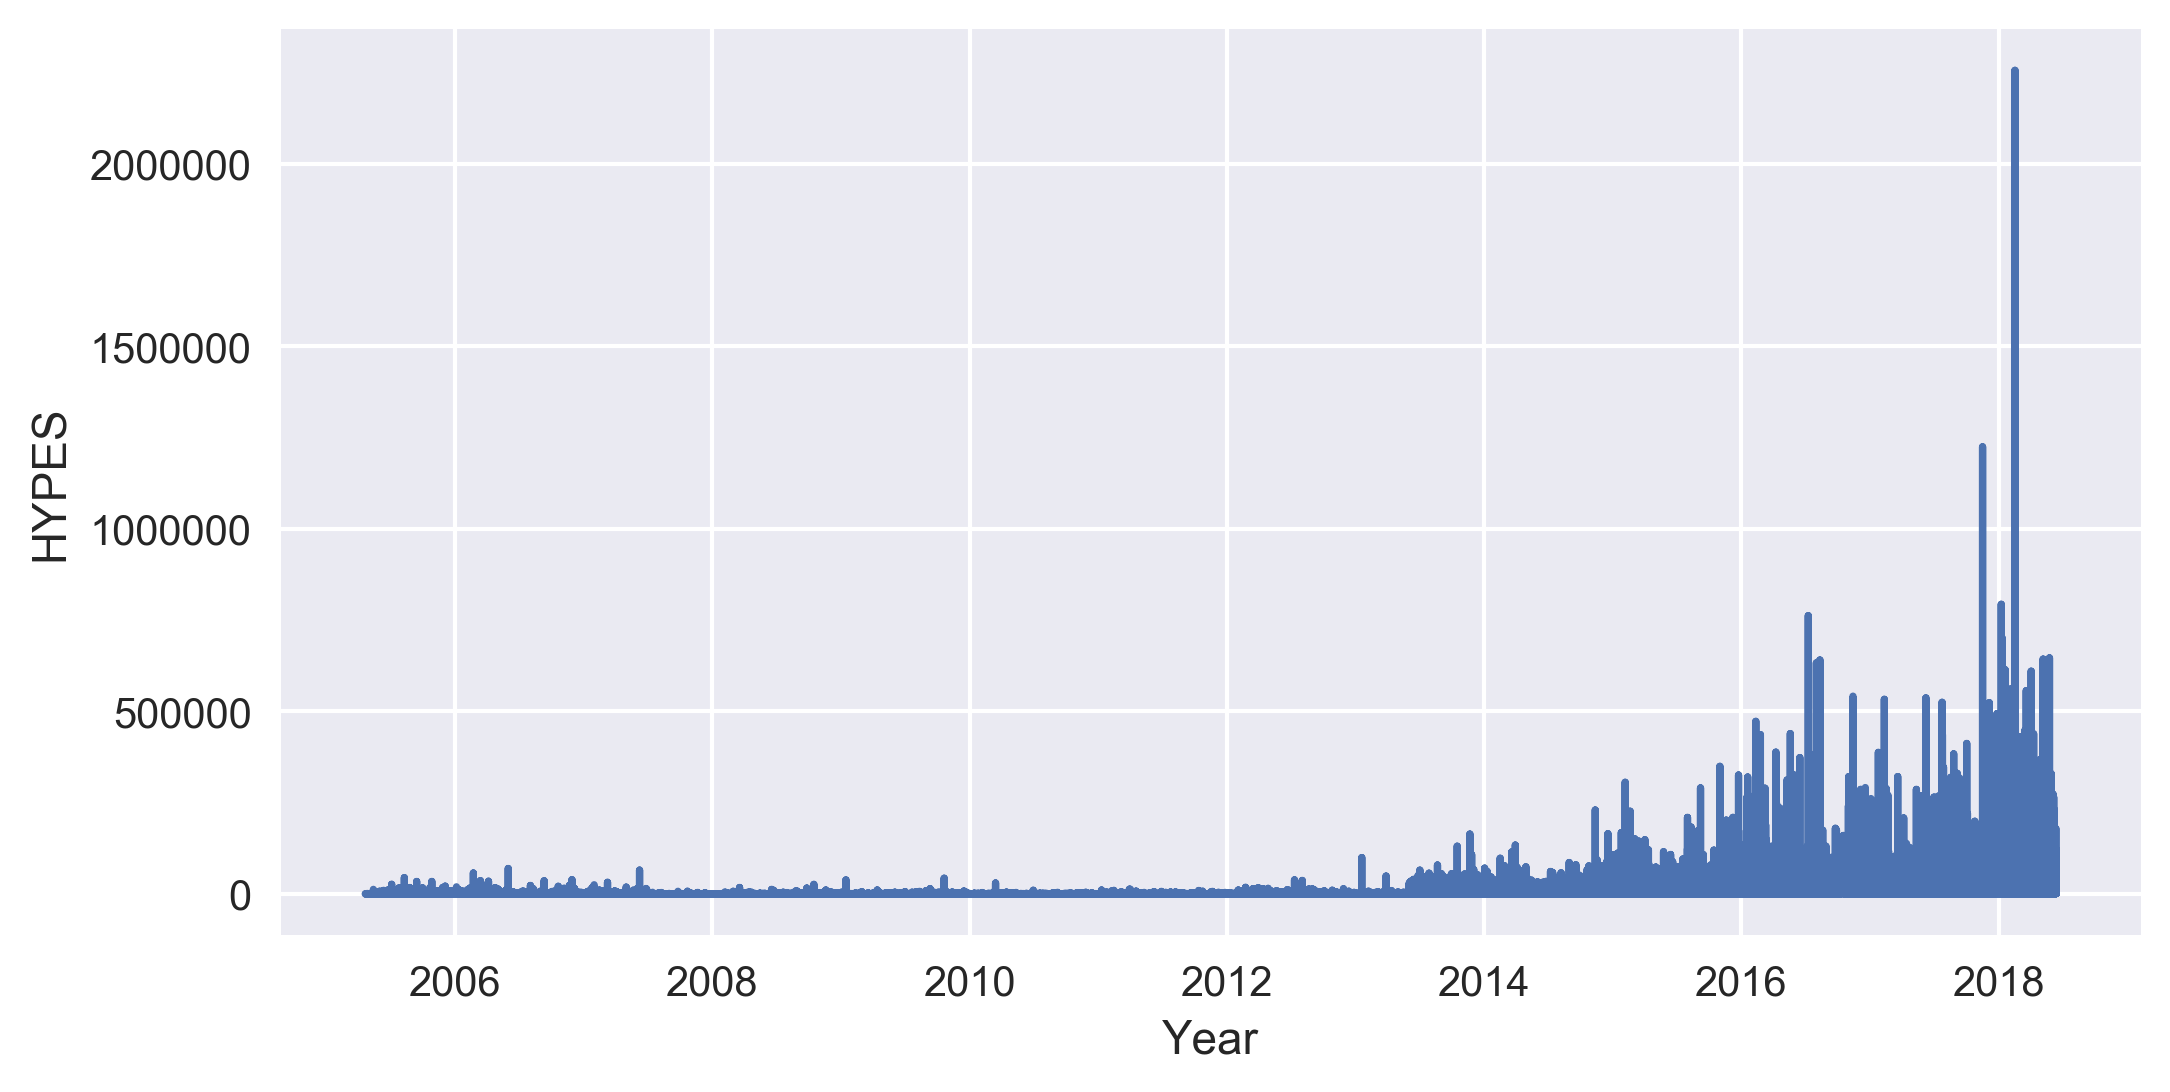
\includegraphics[width=0.9\textwidth]{hypes_year.png}
\caption{HYPES over years}
\label{hypes_yeas}

\end{figure}

\begin{figure}
\centering
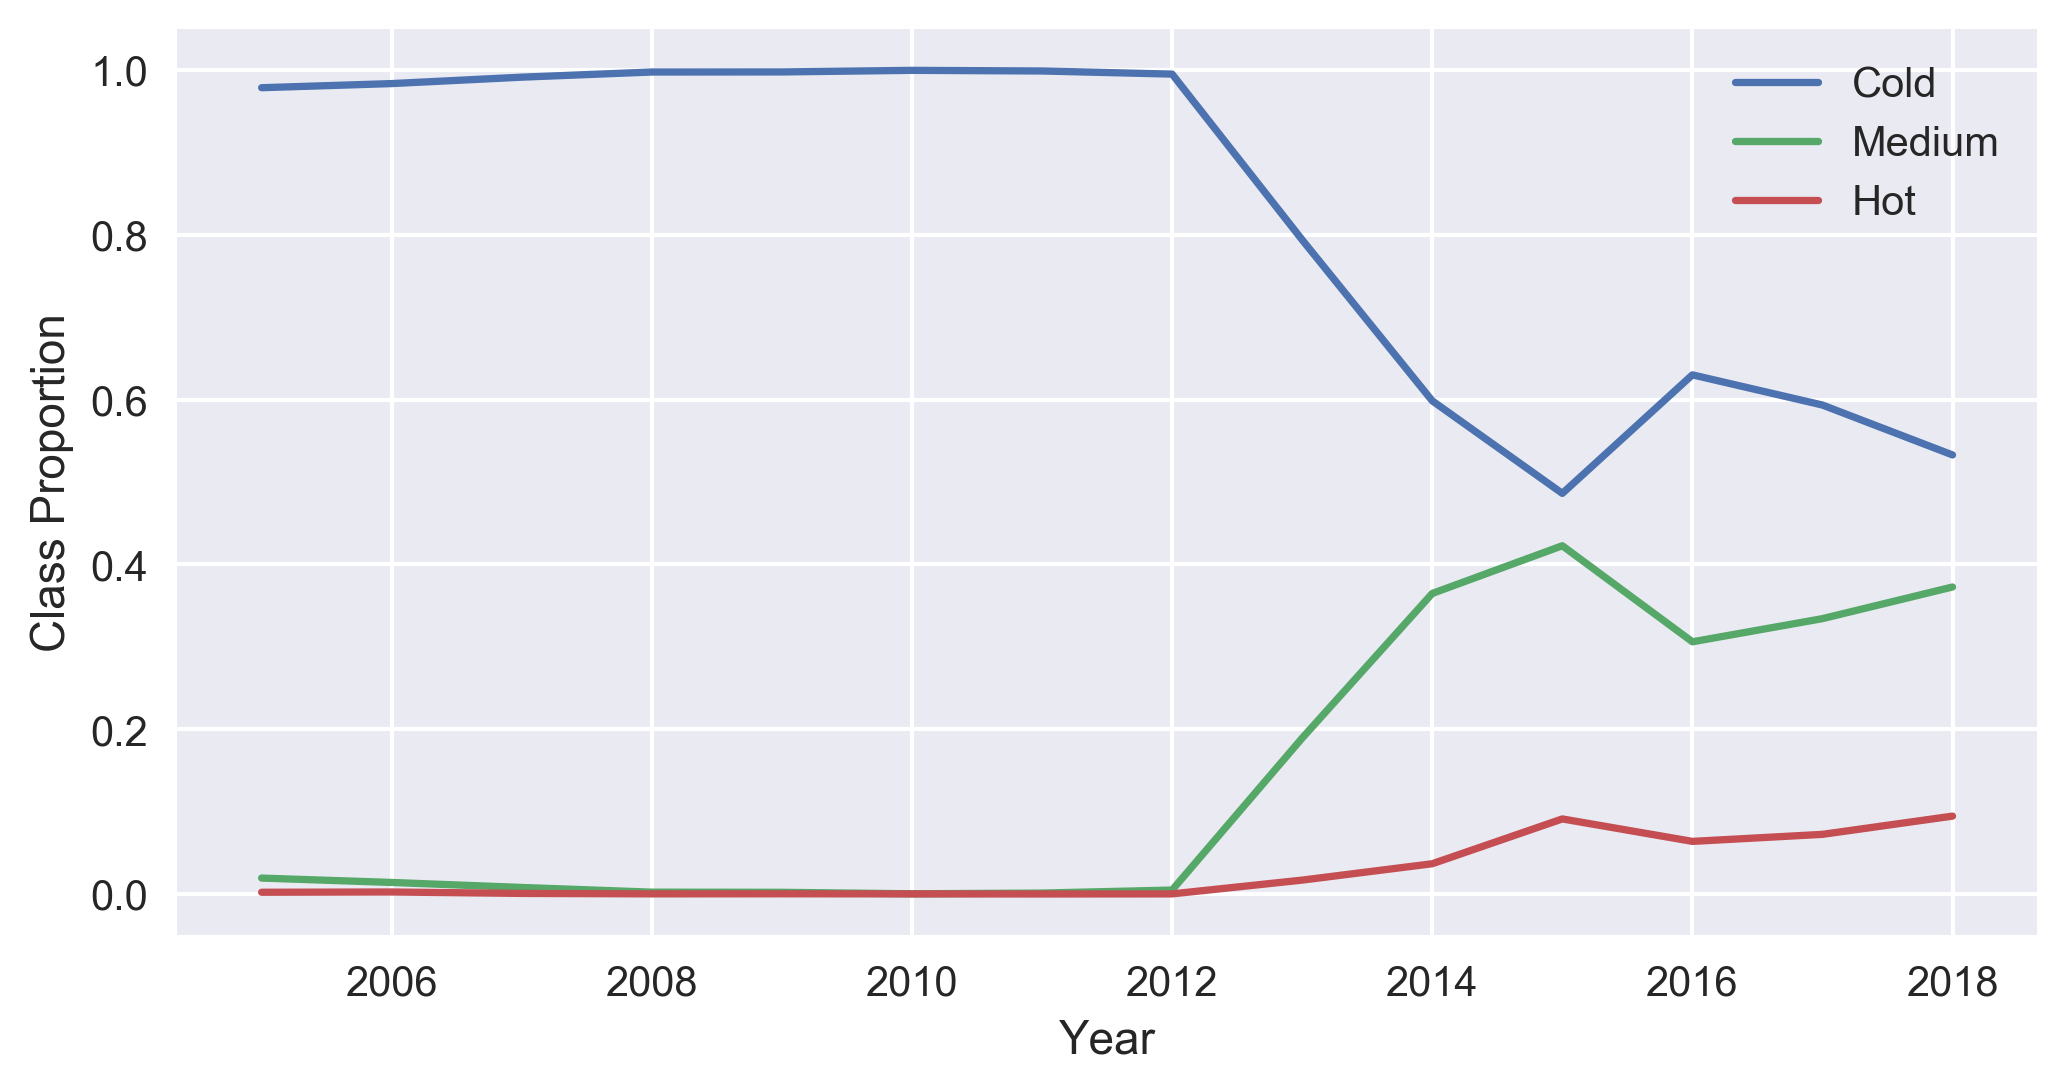
\includegraphics[width=0.9\textwidth]{proportion_hypes.png}
\caption{Proportion of each class over years}
\label{proportion_yeas}
\end{figure}


\begin{table}[]
\centering
\begin{tabular}{lll}
\multicolumn{1}{c}{Popularity} & \multicolumn{1}{c}{Number} & Proportion \\ \hline
Cold                           & 52852                      & 0.5518     \\
Meidum                         & 35944                      & 0.3752     \\
Hot                            & 6991                       & 0.0730    
\end{tabular}
\caption{Distribution of classes of the dataset}
\label{distribution_classes}
\end{table}




\section{Model Design}
As shown in Figure UNKNOWN, the model proposed in this experiment contains three components: (1) a pre-process part that extract features from raw text; (2) a base learner that gives a prediction with a subset of examples; (3) a concept drift detection algorithm which detects the drift and select the subset of the example to re-train the base learner. These components will be presented in detail in this section.

\subsection{Preprocessing}
Before the training data can be fed to the model, it needs to be transformed to a format the model can understand which is called preprocessing including tokenization, vectorization, and feature selection. The scheme of the pre-processing is shown in Figure UNKNOWN.

In natural language processing problem, tokenization is the procedure of splitting a text into words, phrases, or other meaningful parts. In the other words, tokenization is kind of segmentation. In conventional machine learning problem, Bag-of-words model is the most popular representation to tokenize the text. In this model, a raw article is represented as a bag of its words. It is a commonly used and also very effective model. However, bag-of-words model ignores the order of the words which leads to the same representations of the sentences ``Kanye loves Kim.'' and ``Kim loves Kanye.''. As an alternative, the bag-of-ngam model is used to store the spatial information. To some extent, bag-of-words is a special type of bag-of-ngram which only counts the unigram. 

For example, in a bag-of-ngrams model, text is represent as a collection of unique ngrams (groups of $n$ adjacent tokens). Consider the text ``The YEEZY BOOST restock gets postponed''. Here, the word unigrams $(n=1)$ are ['The', `YEEZY', `BOOST', `restock', `gets', `postponed'] and the bag-of-bigrams $(n=2)$ is ['The YEEZY', `YEEZY BOOST', `BOOST restock', `restock gets', `gets postponed']. 

In this experiment, we tokenize the text into both unigrams and bigrams which not only consider the distribution of the words but also the local connection between the words. Thus, the tokenization result of the sentence aforementioned is 
\begin{lstlisting}[language=Tex,basicstyle = \ttfamily, breaklines = true]
['The', `YEEZY', `BOOST', `restock', `gets', `postponed', 'The YEEZY', `YEEZY BOOST', `BOOST restock', `restock gets', `gets postponed']
\end{lstlisting}

After the tokenization,the ngrams need to be truned into numerical vectors which can be processed by the machine learning algorithm. Firstly, every ngram is assigned a unique index which ranges from 0 to the number of ngrams in the corpus. The example below shows the indexes assigned to the unigrams and bigrams generated for two sentences.

\begin{lstlisting}[language=Tex,basicstyle = \ttfamily, breaklines = true]
Raw texts: 
	`Where to buy the YEEZY BOOST.'
	`Your first look at the YEEZY BOOST.'
Index assigned for every ngrams: 
	{'Where': 7, `to': 6, `buy': 2, `the': 5, `YEEZY': 8, `BOOST': 1, `You': 9, `first': 3, `look': 4, `at': 0}
\end{lstlisting}

Once the indexes are siggned to the ngrams, we vectorize using the encoding methods. There are three popular encoding methods. The first one is the one-hot coding by which the text is represented as a vector indicating the presence or absence of a token in the text. The second one is the count encoding by which the text is encodded as a vector indicating the count of a ngrams. The disadvantage of the above two methods is that common words such as `the', `and' are not pernalized. These words occurs in similar frequencies in all texts and are not particularly unique to the text samples in the dataset. Thus, in our model, we use the tf-idf encoding to represent the ngrams. $\mbox{tf}$ means term frequency and $\mbox{idf}$ means inverse document frequencey. The formula used to compute the tf-idf of ngrams is that
\begin{equation}
\mbox{tf-idf}(d,t) = \mbox{tf} * \mbox{idf}(d,t)
\end{equation}
and the $\mbox{idf}$ is computed as 
\begin{equation}
\mbox{idf}(d,t) = \mbox{log} (\frac{n}{\mbox{df}(d,t)}) +1
\end{equation}
where $n$ is the total number of documents and $\mbox{df}(d,t)$ is the document frequency which is defined as the number of documents $d$ that contain term $t$. The constant `$1$' is added to make the terms with zero $\mbox{idf}$ will not be entirely ignored. tf-idf helps to ajust for the fact that some words appear more frequently in general.

During above process, we also apply some tricks. One of them is the lowercase conversion. Since uppercase or lowercase forms words are assumed to have no difference. Another is the stop-words removal. The stop-words are usually assumed to be irrelevant in text classification~\cite{uysal2014impact}.

The vectorized feature vectors are alway high-dimensional in text classification problem because the size of the corpus is very large. In addition, not every feature extracted from the text is useful for the classification. In this case, feature selection is a necessary step which is helpful (1) to improve the performance of the classifier and avoid the overfitting; (2) to reduce the memory storage and provide a more cost-effective model (3) to gain a deeper insight into the underlying processes that generated the data. 

If the features are categorical, we normally calculate a chi-square statistic between each feature and the target vector. However, the encoded features are quantitative. Therefore, we select the features by computing the ANOVA F-value between each feature and the target vector. The F-val scores examine if, when we group the numerical features by the target vectors, the means for each group are significantly different. Based on F-val scores, we can remove the features so as are statistically uncorrelated with class labels.

Suppose the encoded feature vectors $\mathbf{X} \in \mathbb{R}^{n\times m}$, where $n$ is the number of examples and $m$ is the number of features, and the labels $\mathbf{Y} \in \mathbb{R}^{n\times l}$, where $l$ is the number of classes. We assume to select $k$ relevant features from $m$ features. Hence, there are $(n \choose k)$ combinations. Then, we compute the F-score for each combination with the ANOVA table and retain the $k$ features from the group with the highest F-score. 


\subsection{Base Learner}
In the experiment, the naive bayes classifier is used as base learner. It is because it naturally support incremental learning which can provide a fast and cost-efficient model.

For a given document $d$ with class of $y$, the Bayes' theorem present the relationship as a follow:
\begin{equation}
P(y|d) = \frac{P(d|y) p(y)}{P(d)}
\end{equation}
As what we mentioned in section of pre-processing, the document $d$ is represented as features $(x_1, x_2,...,x_k)$. The Naive Bayes method using a strong and naive assumption that the feature probabilities $P(x_i|y_j)$ are independent given the class $y$. Hence, the relationship is simplified to

\begin{equation}
\begin{aligned}
P(y|d) & = p(y|x_1,...,x_k) \\
	   & = \frac{P(y)P(x_1,..x_k|y}{P(x_1,..,x_k)}\\
	   & = \frac{P(y)\prod_{i=1}^kP(x_i|y)}{P(x_1,...,x_k)}\\
	   & \propto P(y)\prod_{i=1}^kP(x_i|y)
\end{aligned}
\end{equation}

The prediction result can be obtained by using the Maximum A Posteriori (MAP)
\begin{equation}
\hat{y} = \mbox{argmax}_y P(y)\prod_{i=1}^kP(x_i|y)
\end{equation}

In the experiment, we use the multinomial naive Bayes algorithm which is commonly used in text classification. The data distribution is parametrized by the vectors $\mathbf{\theta}_y = (\theta_{y_1}, ..., \theta_{y_k})$ for each class $y$, where $\theta_{y_i}$ is the probability $P(x_i|y)$ which is estimated as

\begin{equation}
\hat{\theta}_{y_i} = \frac{N_{y_i} + \alpha}{N_y+\alpha k}
\end{equation}

where $N_{y_i}$ is the number of times feature $i$ appears in a sample of class $y$ in the training set and $N_y$ is the total count of all features for class $y$.

The hypeparameter $\alpha$ is the smoothing parameter which incorporate a small-sample correction. It is a type of regularization. When a given test point whose class and one of features never occur together in the training set, the estimated probability will be zero. Because of the multiplication, the posteriori will be zero. Thanks to the smoothing parameters, no probability is set to zero. When $\alpha=1$, the smoothing is called Laplace smoothing, and Lidstone smoothing in the general case.

\subsection{Concept Drift Detection Algorithm}

In the experiment, we use Drift Detection Method (DDM) proposed by Gama et al.~\cite{gama2004learning}. Previous experiments have prove that DMM has the best performance in both gradual and abrupt drift~\cite{Goncalves2014}. In addition, compared with other detector, DMM is relative fast and cost-efficient. 

DMM was proposed by the probably approximately correct learning model~\cite{michalski2013machine} that if the distribution of the data is stationary, the error rate of the classifier will decrease with the increase of the number of the instances. Therefore, a great increase of the error rate indicates the change of the distribution, namely, the concept drift. 

For every instance at time $i$, the error-rate $p_i$ and the standard deviation $s_i = \sqrt{p_i(1-p_i)}$ are computed. $p_{min}$ and $s_{min}$ are stored when $p_i$ and $s_i$ reach their minimum. A warning level is reached if $p_i + s_i \geq p_{min} + \alpha \cdot s_{min} $ and a drift occurs when $p_i + s_i \geq p_{min} +\beta \cdot s_{min}$, where $\alpha$ and $\beta$ are number of standard deviation to warn ($\alpha$) and detect ($\beta$) drift. With confidence levels for warning and drift set to 95\% and 99\% respectively, $\alpha$ is $2$ and $\beta$ is $3$. When a warning level is reached, the instances after the warning level are stored. Once the drift occurs, the base learner will re-trained by the stored instance and the values of $p_{min}$ and $s_{min}$ will be reset. It often happens that the error rate increases and reach the warning level but decrease later. It is called false alarm. Once the false alarm occurs, the stored instances will be thrown away. Based on this mechanism, DDN keeps the base learner better adapted to the present data distribution.

DMM can be applied to any machine learning algorithm. It can be directly implemented inside the incremental learning algorithm and also can be implemented as a wrapper to batch learner. In this experiment, the DMM is implemented as a wrapper over the multinomial Bayes classifier that incrementally learns the dataset. Figure UNKOWN presents the process at time $i$


%\begin{algorithm}
%\caption{DMM with Bayes Classifier}
%\label{ddm}
%\begin{algorithmic}
%\REQUIRE ~~\\
%$\Phi$: Current Bayes Classifier \\
%$\mathbf{x}_i, y_i$: Current example
%\Begin
%Let $\hat{y_i} \leftarrow \Phi(\mathbf{x}_i)$
%Compute $p_i$ and $s_i$
%\IF{$p_i + s_i < p_{min} + s_{min} $}
%\STATE $p_min \leftarrow p_i$ 
%\STATE $s_min \leftarrow s_i$ 
%\ENDIF
%\end{algorithmic}
%\end{algorithm}

\subsection{Evaluation Step}
To evaluate the performance of the concept drift detector, we use an approach described by Elwell et al.~\cite{Elwell2011}. For each time $t$, the instance from time $t+1$ is used as the test data. We assume $T$ as the time step. For each time step $T$, there are specific amount of test instances. Then, a variety of metrics is computed for each time step to compared the performance between the concept drift detector and the base learner. 

Firstly, we focus on the basic metric, the accuracy. For each test instance, the Bayes Classifier will return a boolean value indicating if it correctly classified the instance or not. For every time step $T$, the accuracy is defined as

\begin{equation}
\mbox{Accuracy} = \frac{\mbox{Number of correctly predicted instance} }{\mbox{Number of instances}}
\end{equation}

However, the data set is imbalanced, the number of hot news is significantly less than other two types of news. High accuracy does not indicate good classification ability. Using accuracy to evaluate the models will drive the models focus on the majority class but ignore the minority. In this case, accuracy alone is typically not enough information to do the comparison. In addition, we expect the hot news can be predicted correctly as much as possible. Thus, the recall is used to check if the model returns most of the relevant result.

For binary classification, recall is intuitively defined as 
\begin{equation}
\mbox{Recall} = \frac{tp}{tp+fn}
\end{equation}
where $tp$ is the number of correctly predicted positive instances, and $fn$ is the predicted correctly negative instance. However, our model is designed to deal with multiclass classification problem. The definitions of true positive ($tf$) and false negative ($fn$) are slightly different. The multiclass problem is separated into several binary classification problem. For class $i$, the true positive $tf_i$ and false negative ($fn_i$) are computed by treating class $i$ as the positive class and other classes are all negative. Then, we compute the micro-average recall as it aggregates the contributions of all classes to compute the average metric. The micro-average recall is defined as~\cite{sokolova2009systematic} 
\begin{equation}
\mbox{micro-Recall} = \frac{\sum_i tf_i}{\sum_i(tf_i + fn_i)}
\end{equation}

In addition, we also compute the micro average F1 score which is the weighted average of micro-average precision and micro-average recall.

\begin{equation}
\mbox{micro-F}_1 = 2 * \frac{\mbox{micro-Precision} * \mbox{micro-Recall}}{\mbox{micro-Precision} + \mbox{micro-Recall}}
\end{equation}

where definition of the micro-average precision is similar to the micro-average recall which is shown as a follow
\begin{equation}
\mbox{micro-Precision} = \frac{\sum_i tf_i}{\sum_i(tf_i + fp_i)}
\end{equation}
where $fp$ is number of negative instances which are predicted as positive.

In addition to pay attention the prediction result of the instances at each time step, the overall performance of the model will be evaluated as well. Apart from accuracy, micro-average recall, and micro-average F1 score, the normalized confusion matrix will be computed and visualized.

\subsection{Parameters Configuration}

\section{Experimental Results}
\subsection{Drift Identification}
\subsection{Predictive Accuracy}